\documentclass{article}
\usepackage{tikz}

\usetikzlibrary{intersections}
\usetikzlibrary{angles, quotes}

\tikzset{help lines/.style=very thin}
\tikzset{Karl's grid/.style={help lines,color=blue!50}}

\begin{document}

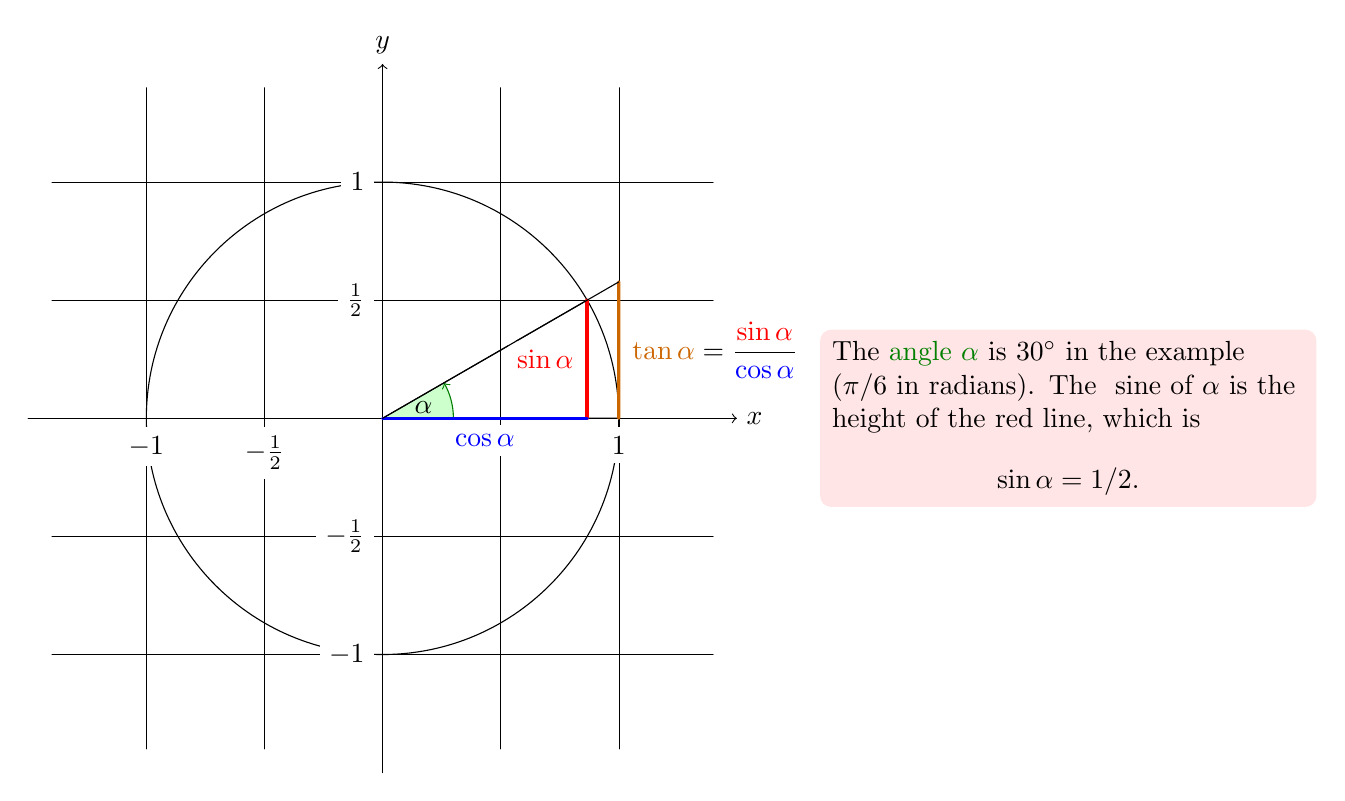
\begin{tikzpicture}
    [scale=3,line cap=round,
    % Styles
    axes/.style=,
    important line/.style={very thick},
    information text/.style={rounded corners,fill=red!10,inner sep=1ex}]

    % Colors
    \colorlet{anglecolor}{green!50!black}
    \colorlet{sinecolor}{red}
    \colorlet{tancolor}{orange!80!black}
    \colorlet{coscolor}{blue}

    % Coordinates
    \coordinate (A) at (1,0);
    \coordinate (B) at (0,0);
    \coordinate (C) at (30:1cm);

    % Graphic
    \draw[help lines, step=0.5cm] (-1.4,-1.4) grid (1.4,1.4);
    \draw (0,0) circle [radius=1cm];

    \begin{scope}[axes]
        \draw[->] (-1.5,0) -- (1.5,0) node[right] {$x$} coordinate(x axis);
        \draw[->] (0,-1.5) -- (0,1.5) node[above] {$y$} coordinate(y axis);

        \foreach \x/\xtext in {-1, -0.5/-\frac{1}{2}, 1}
            \draw[xshift=\x cm] (0pt, 1pt) -- (0pt, -1pt) node[anchor=north, fill=white] {$\xtext$};
        \foreach \y/\ytext in {-1, -0.5/-\frac{1}{2}, 0.5/\frac{1}{2}, 1}
            \draw[yshift=\y cm] (1pt, 0pt) -- (-1pt, 0pt) node[anchor=east, fill=white] {$\ytext$};
    \end{scope}

    \draw (A) -- (B) -- (C)
        pic [->, draw=green!50!black,
             fill=green!20,
             angle radius=9mm,
             "$\alpha$"]
        {angle = A--B--C};
  
    % \filldraw[fill=green!20,draw=green!50!black] (0,0) -- (3mm,0mm)
    %   arc [start angle=0, end angle=30, radius=3mm] -- cycle;
  
    \draw[important line, sinecolor]
        (30:1cm) -- node[left=1pt, fill=white] {$\sin \alpha$}+(0,-0.5);
    \draw[important line, coscolor]
        (30:1cm |- x axis) -- node[below=2pt,fill=white] {$\cos \alpha$} (0,0);

    \path [name path=upward line] (1,0) -- (1,1);
    \path [name path=sloped line] (0,0) -- (30:1.5cm);
    \draw [name intersections={of=upward line and sloped line, by=x}]
          [important line, tancolor] (1,0) -- node[right=1pt, fill=white] 
          {$\displaystyle \tan \alpha \color{black} = \frac{\color{red}\sin \alpha}{\color{blue}\cos \alpha}$} (x);

    \draw (0,0) -- (x);

    \draw[xshift=1.85 cm]
        node [right, text width=6cm, information text]
        {
            The {\color{anglecolor} angle $\alpha$} is $30^{\circ}$ in the example ($\pi/6$ in radians). The {\color{sinecolor}} sine of $\alpha$ is the height of the red line, which is
            \[
                \sin \alpha = 1/2.
            \]
        };


\end{tikzpicture}


\end{document}